\section{Technische Dokumentation}

\subsection{Einleitung}

Die generelle Zielsetzung sah die Erstellung eines Tools vor, das auf Grundlage von Benutzerpräferenzen personalisierte Reisevorschläge erstellt. Nutzer sollten in der Lage sein, Konten zu führen und ihre Reisen zu speichern.
Zusätzlich sollte – nach Möglichkeit – das Tool durch eine anschließende Datenanalyse, bzw. eine Datenvisualisierung erweitert werden.  

\subsection{Architekturübersicht}

\begin{figure}[h]
  \centering
  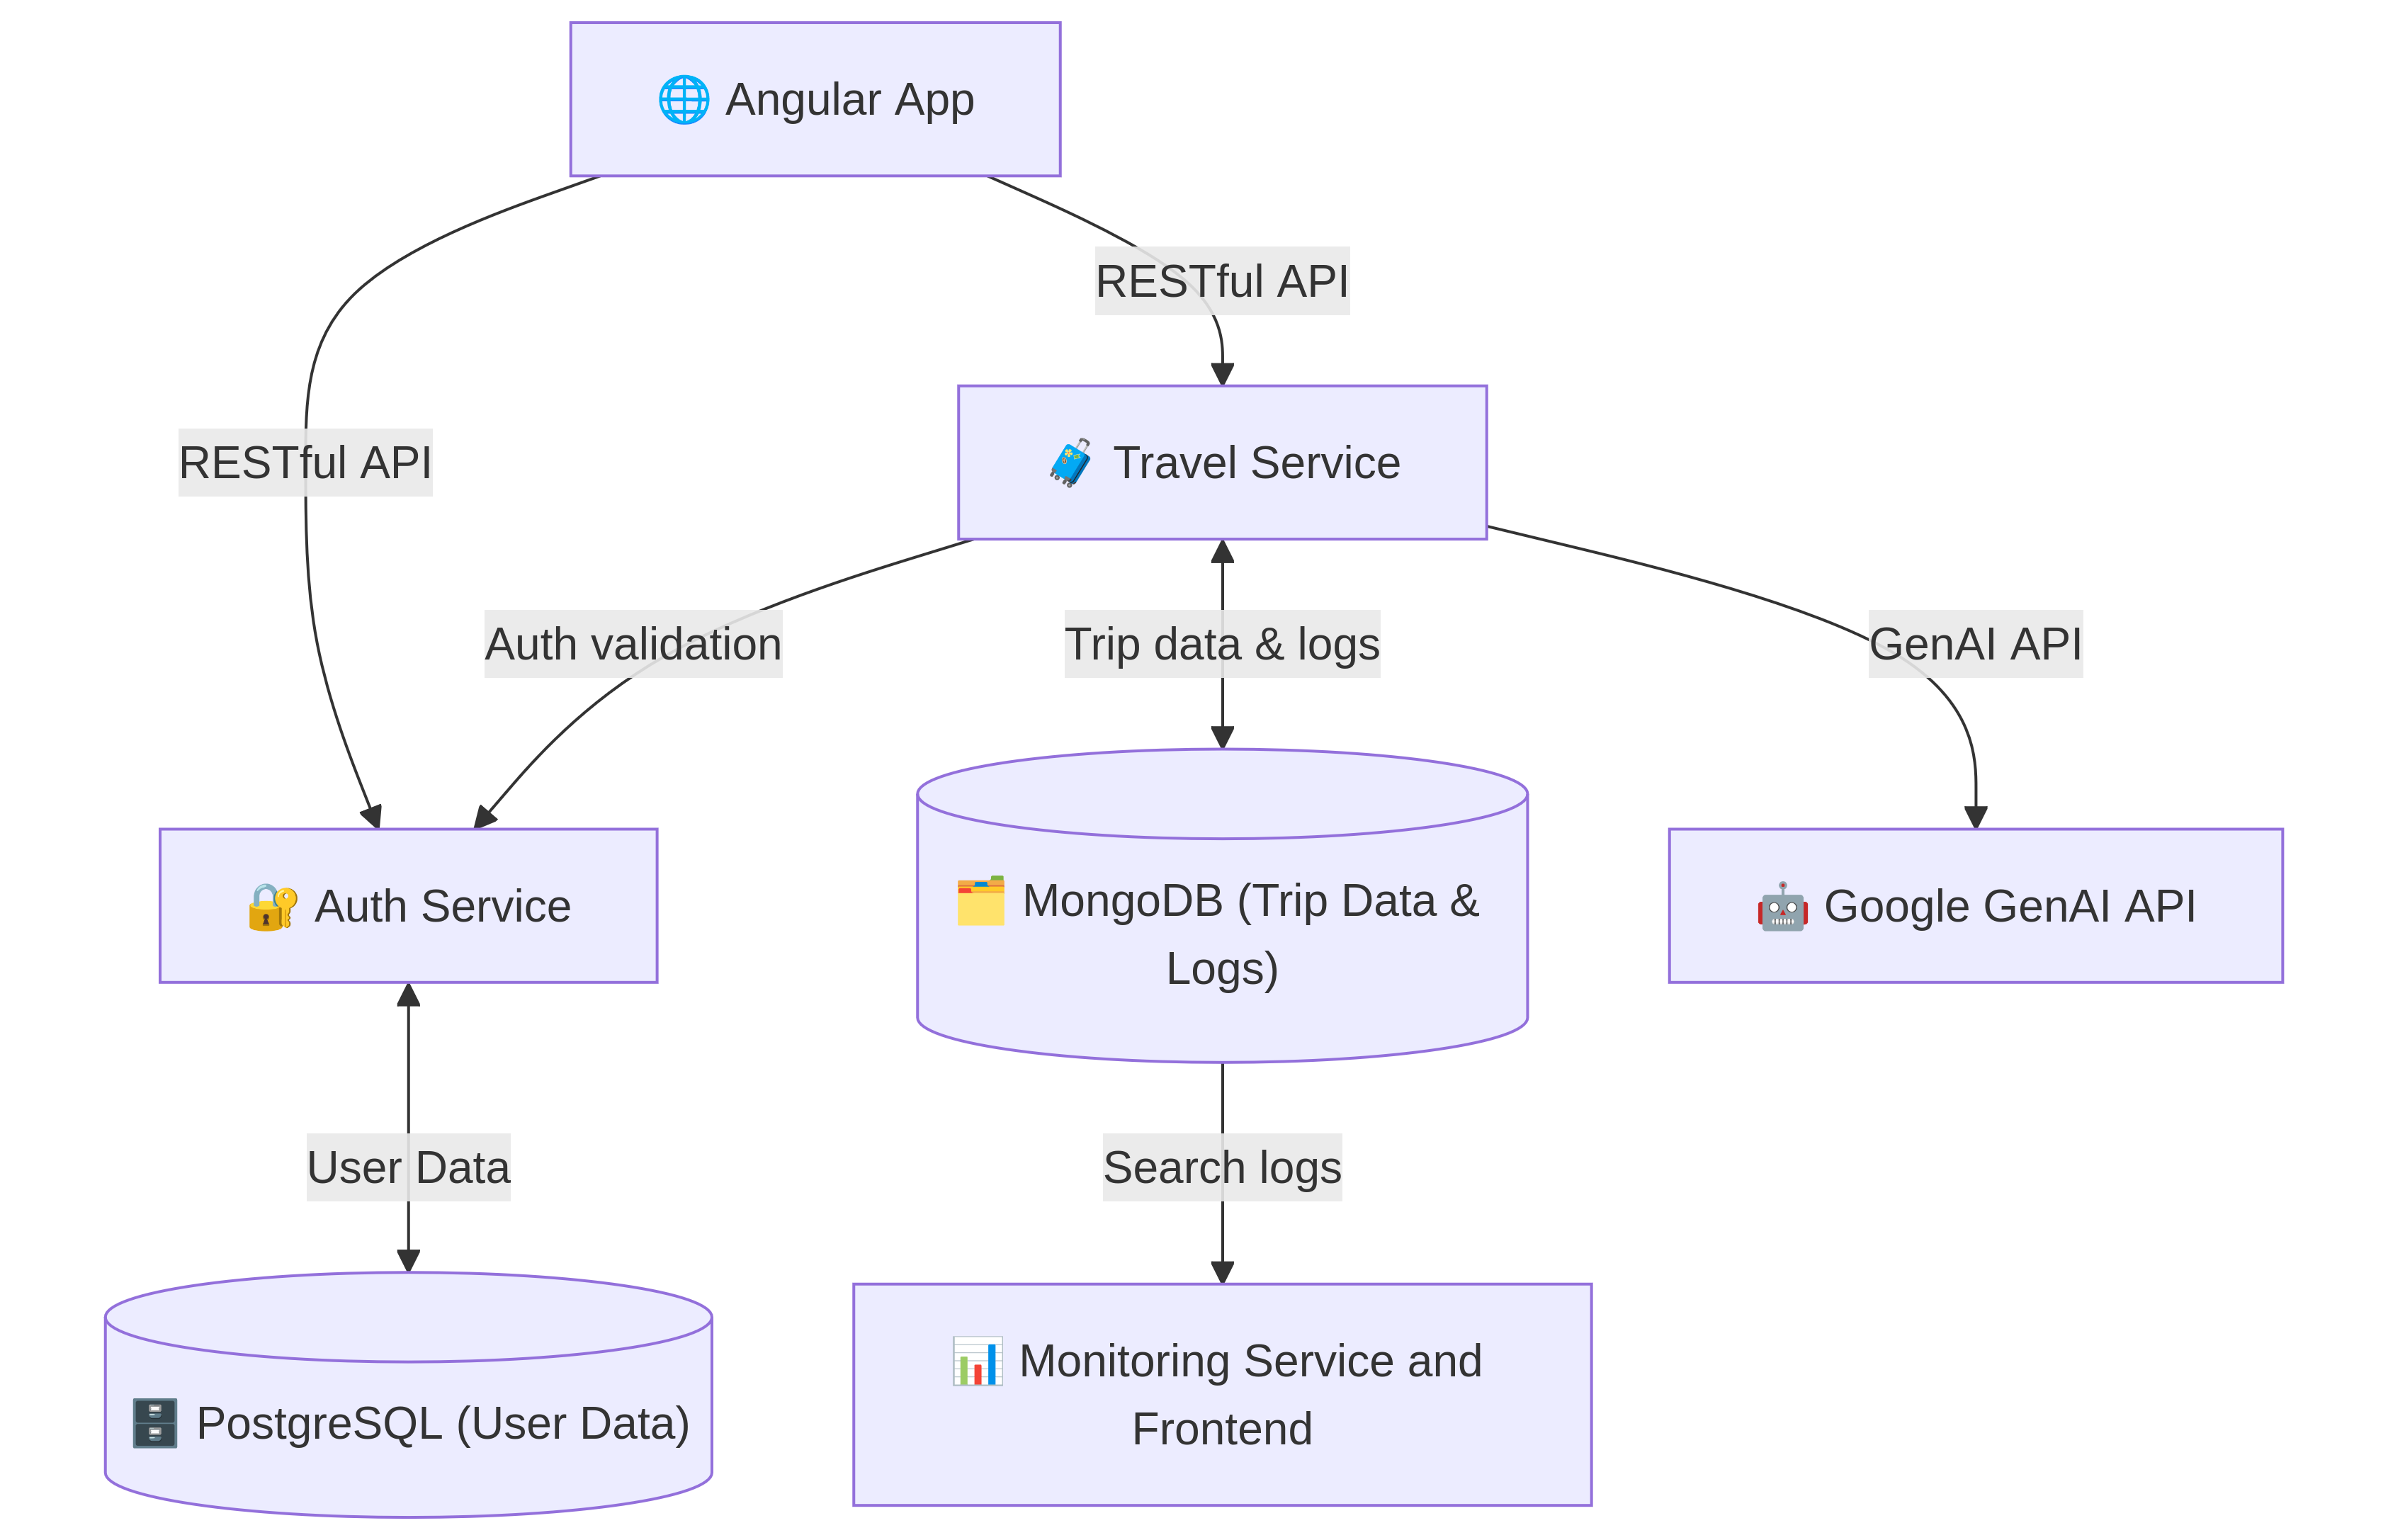
\includegraphics[width=0.8\textwidth]{images/architecture.png}
  \caption{Architekturübersicht des verteilten Systems}
\end{figure}

Die Abbildung zeigt die Architektur des entwickelten Systems. Man sieht hier ganz oben das Frontend, das mit Angular umgesetzt wurde. Es kommuniziert über REST-APIs mit zwei Microservices. Diese Microservices sind der Authentifizierungsservice und der Travel-Planner-Service. Es werden Datenbanken benutzt, um Nutzerdaten, Reisedaten und Log-Daten zu speichern. Für die Logik wird eine externe API von Google GenAI für die Generierung von Reiseempfehlungen eingebunden.

Das Backend ist in zwei separate Microservices unterteilt:
\begin{itemize}
  \item \textbf{auth\_service}: übernimmt die Authentifizierung und Verwaltung von Nutzerkonten und Präferenzen
  \item \textbf{travel\_service}: verarbeitet Nutzeranfragen, verwaltet geplante Reisen und generiert personalisierte Empfehlungen
\end{itemize}

Abschließend wurden sämtliche Anwendungen containerisiert und über ein Kubernetes-Cluster orchestriert. Dies ermöglicht eine standardisierte, skalierbare und portable Bereitstellung der Anwendung.


\subsection{Frontend}

Wie in der Vorlesung vorgestellt, wird hier auch Angular als Framework für die Frontend-Entwicklung eingesetzt. Angular basiert auf einem MVC-Pattern, das eine klare Trennung von Logik, Daten und Darstellung ermöglicht.
Konkret bei Angular werden Models durch die Typescript-Interfaces und Angular Services realisiert. Die Views werden durch HTML-Templates und CSS-Stile definiert, während die Controller-Logik in TypeScript-Klassen implementiert wird. Diese Struktur lässt den Code sehr gut modularisieren.

Angular eignet sich in diesem Fall besonders gut, da es eine reaktive Programmierung unterstützt und somit eine dynamische Benutzeroberfläche ermöglicht. Die Kommunikation mit den Backend-Microservices erfolgt über REST-APIs, die JSON-Daten austauschen, was ein guter Standard ist und ohne Probleme in verteilten Systemen funktioniert.

\subsubsection{Komponenten}
Die Angular-Anwendung besteht aus mehreren Komponenten, die jeweils für bestimmte Funktionalitäten zuständig sind. Die wichtigsten Komponenten sind:

\begin{itemize}
  \item \textbf{LoginComponent}: Ermöglicht die Anmeldung von Nutzern
  \item \textbf{RegisterComponent}: Ermöglicht die Registrierung neuer Nutzer
  \item \textbf{HomeComponent}: Zeigt die Startseite mit gespeicherten Reisen an
  \item \textbf{TripComponent}: Zeigt Details zu geplanten Reisen an.
  \item \textbf{RecommendationsComponent}: Ermöglicht die Eingabe von Reisepräferenzen und zeigt generierte Empfehlungen an. Später lässt sich hier auch eine Reise speichern.
\end{itemize}

Jeder dieser Komponenten hat eine eigene HTML-Template-Datei, die das Layout definiert, sowie eine TypeScript-Datei, die die Logik und Interaktion mit den Backend-Services implementiert. Die Kommunikation mit den Microservices erfolgt über Angular Services, die HTTP-Anfragen an die REST-APIs senden und die Antworten verarbeiten.

\subsubsection{Angular Services}

Die Angular-Anwendung nutzt Services, um die Kommunikation mit den Backend-Microservices zu abstrahieren. Diese Services kapseln die HTTP-Anfragen und ermöglichen eine einfache Wiederverwendbarkeit der Logik in verschiedenen Komponenten.
Hier gibt es drei zentrale Services:

\begin{itemize}
  \item \textbf{AuthService}: Verwaltet die Authentifizierungvon Nutzern, indem er mit dem Authentifizierungsservice kommuniziert. Er stellt Methoden zum Anmelden, Registrieren und Abrufen von Benutzerdaten bereit.
  \item \textbf{SuggestionService}: Kommuniziert mit dem Travel-Planner-Microservice, um Reiseempfehlungen zu generieren und geplante Reisen zu verwalten.
  \item \textbf{TripService}: Ist für das Abrufen und Speichern von Reisedaten zuständig.
\end{itemize}

Außerdem ist ein Interceptor implementiert, der alle HTTP-Anfragen abfängt und den JWT-Token für die Authentifizierung an die Header anhängt. Dies ermöglicht eine sichere Kommunikation mit den Microservices, ohne dass der Token manuell in jeder Anfrage hinzugefügt werden muss.


\subsection{Microservice-Architektur}

Das Backend wurde mithilfe von FastAPI in zwei Microservices umgesetzt. Die Architektur folgt dem Prinzip der Modularisierung und entspricht dem in der Vorlesung behandelten Aufbau verteilter Systeme.

\subsubsection{Containerisierung mit Docker}

Beide Microservices wurden containerisiert und in einem Docker-Setup betrieben. Aufbau, Build und Deployment der Container orientieren sich an den in der Vorlesung vermittelten Grundlagen.

\subsubsection{Kubernetes Cluster}

Die containerisierten Microservices wurden in einem Kubernetes-Cluster orchestriert. Damit wurde ein praxisnaher Anwendungsfall der in der Vorlesung behandelten Themen zu Skalierung und Verwaltung verteilter Systeme umgesetzt.

\subsubsection{Authentifizierungs-Microservice}

Der entwickelte Authentifizierungs-Microservice dient der Verwaltung von Benutzerkonten sowie der Authentifizierung registrierter Benutzer. Ziel ist es, auf Grundlage einer sicheren und überprüfbaren Identität weitere Microservices – insbesondere den Travel-Planner-Service – vor unberechtigtem Zugriff zu schützen. Die Implementierung erfolgt auf Basis des Python-Webframeworks FastAPI, das sich insbesondere durch seine hohe Performance, asynchrone Unterstützung und einfache OpenAPI- Integration (Swagger UI) auszeichnet. Letztere ermöglicht die einfache Interaktion mit den bereitgestellten REST-Endpunkten.

Zur Datenvalidierung kommt Pydantic v2 zum Einsatz. Diese Bibliothek erlaubt eine deklarative Modellierung und Validierung von Datenstrukturen auf Basis von Python-Typannotationen. Durch Pydantic wird sichergestellt, dass Nutzerdaten wie E-Mail-Adresse, Passwort und vollständiger Name beim Eintreffen überprüft und ggf. abgewiesen werden, bevor sie weiterverarbeitet werden. Dies stellt eine zentrale Maßnahme zur Stärkung der Systemsicherheit dar.

Die Speicherung von Passwörtern erfolgt unter Verwendung des bcrypt-Algorithmus, einem bewährten Verfahren zur sicheren und einwegigen Hashing-Verarbeitung sensibler Daten. Bcrypt schützt insbesondere gegen Brute-Force-Angriffe und Rainbow-Table-Attacken.

Für die Authentifizierung wurde ein JWT-basiertes (JSON Web Token) Verfahren implementiert. Beim erfolgreichen Login wird ein signierter Token generiert, der die Identität des Nutzers in Form eines sogenannten Claims (z.B. die E-Mail-Adresse) enthält. Dieser Token kann anschließend von anderen Microservices – z.B. dem Travel Planner – zur Authentifizierung des Nutzers verwendet werden, ohne dass das Passwort erneut übertragen werden muss. Damit wird das Prinzip der stateless Authentication umgesetzt, was insbesondere in verteilten Systemarchitekturen von Vorteil ist.

Die Benutzerinformationen werden in einer PostgreSQL-Datenbank persistiert. PostgreSQL wurde aufgrund seiner Zuverlässigkeit, Transaktionssicherheit und guten Integration in Python-Projekte ausgewählt.

Die gesamte Systemarchitektur orientiert sich am HATEOAS-Prinzip (Hypermedia as the Engine of Application State). Dadurch werden dem Client über die API nicht nur Daten, sondern auch Informationen über mögliche nächste Schritte zur Verfügung gestellt. Dies trägt zu einer entkoppelten, wartbaren Struktur bei und erleichtert die Integration mehrerer Microservices.

\subsubsection{User Gruppen}

In unserem System gibt es verschiedene Benutzergruppen, die unterschiedliche Funktionen nutzen.

Die Hauptnutzergruppe besteht aus Endnutzern, zum Beispiel Familien oder Einzelpersonen, die auf einfache Weise eine Reise planen möchten. Diese Nutzer können sich passende Reiseziele vorschlagen lassen, basierend auf ihren persönlichen Präferenzen. Darüber hinaus besteht die Möglichkeit, Reisen zu speichern, um später erneut darauf zugreifen zu können. Neben konkreten Zielen lassen sich auch Aktivitäten für die geplante Reise anzeigen.

Zusätzlich existieren administrative oder technische Nutzer, die über einen separaten Monitoring-Service Zugriff auf Systemdaten und Nutzungsinformationen erhalten. Dieser Service dient der Analyse und Kontrolle des Gesamtsystems.

\subsubsection{Geschäftsprozesse}

Im Projekt wurden drei zentrale Geschäftsprozesse abgebildet: die Registrierung, die Authentifizierung (Login) und die Reisesuche mit optionaler Speicherung.

Bei der Registrierung werden Benutzerdaten wie E-Mail, Passwort und Name über das Frontend erfasst und an den Authentication-Microservice übergeben. Dort erfolgt mithilfe der Bibliothek Pydantic v2 eine Datenvalidierung, wodurch Eingabefehler frühzeitig erkannt werden. Das Passwort wird mit dem sicheren Hashing-Verfahren bcrypt verschlüsselt und anschließend in einer PostgreSQL-Datenbank gespeichert.

Beim Login wird der Nutzer erneut über E-Mail und Passwort authentifiziert. Bei erfolgreicher Anmeldung wird ein sogenannter JWT-Token (JSON Web Token) erstellt und dem Nutzer übermittelt. Dieser Token dient als Identitätsnachweis und wird bei nachfolgenden Anfragen an andere Microservices verwendet, um den Nutzer zu identifizieren.

Ein weiterer zentraler Prozess ist die Reisesuche. Nach erfolgreicher Authentifizierung kann der Nutzer über das Frontend individuelle Wünsche und Kriterien für seine Reise eingeben. Diese Informationen werden an den Travel-Planner-Microservice übergeben. Dieser analysiert die Daten mithilfe des Sprachmodells Gemini und generiert daraufhin passende Reisezielvorschläge. Die Ergebnisse werden im Frontend ausgegeben. Nutzer haben anschließend die Möglichkeit, eine Reise dauerhaft zu speichern. Dabei wird mithilfe des JWT-Tokens überprüft, ob der Nutzer angemeldet ist. Die Reiseinformationen werden dann in einer MongoDB-Datenbank abgelegt und mit einer eindeutigen Nutzerkennung verknüpft. Auf diese Weise ist sichergestellt, dass jeder Nutzer nur Zugriff auf seine eigenen gespeicherten Reisen hat.

Zur Umsetzung dieser Prozesse wurden gezielt technische Maßnahmen gewählt, die die Anforderungen des Systems effektiv unterstützen. Die Nutzung von FastAPI als Framework ermöglicht eine schnelle und effiziente Entwicklung der REST-Schnittstellen. Durch die Integration von Swagger UI kann die API direkt getestet werden, was insbesondere während der Entwicklung und im Austausch mit anderen Projektteilen von Vorteil ist. Die Kombination aus JWT-basiertem Login, bcrypt zur Passwortverschlüsselung sowie einer klaren Trennung zwischen Authentifizierung und Anwendungslogik über Microservices trägt zur Sicherheit und Skalierbarkeit des Systems bei. Die Datenvalidierung über Pydantic sorgt für Robustheit und reduziert Fehlerquellen bereits bei der Eingabe.

\subsection{Kompromisse und Abweichungen}
